\documentclass[11pt,a4paper]{article}
\usepackage{diagbox}
\usepackage{wrapfig}
\usepackage[utf8]{inputenc}
%\usepackage[swedish]{babel}
\usepackage{graphicx}
\usepackage{amsmath}
\usepackage{amssymb}
\usepackage{units}
\usepackage{ae}
\usepackage{icomma}
\usepackage{color}
\usepackage{graphics} 
\usepackage{bbm}
\usepackage{float}

\usepackage{caption}
\usepackage{subcaption}

\usepackage{hyperref}
\usepackage{epstopdf}
\usepackage{epsfig}
\usepackage{braket}
\usepackage{pdfpages}

\usepackage{tcolorbox}

\newcommand{\N}{\ensuremath{\mathbbm{N}}}
\newcommand{\Z}{\ensuremath{\mathbbm{Z}}}
\newcommand{\Q}{\ensuremath{\mathbbm{Q}}}
\newcommand{\R}{\ensuremath{\mathbbm{R}}}
\newcommand{\C}{\ensuremath{\mathbbm{C}}}
\newcommand{\id}{\ensuremath{\,\mathrm{d}}}
\newcommand{\rd}{\ensuremath{\mathrm{d}}}
\newcommand{\Ordo}{\ensuremath{\mathcal{O}}}% Stora Ordo
\renewcommand{\L}{\ensuremath{\mathcal{L}}}% Stora Ordo
\newcommand{\sub}[1]{\ensuremath{_{\text{#1}}}}
\newcommand{\Vp}{\ensuremath{\mathcal{V}'} }
\newcommand{\ddx}[1]{\ensuremath{ \frac{\partial}{\partial #1} }}
\newcommand{\ddxx}[2]{\ensuremath{ \frac{\partial^2}{\partial #1 \partial #2} }}
%\newcommand{\sup}[1]{\ensuremath{^{\text{#1}}}}
\renewcommand{\b}[1]{\ensuremath{ {\bf #1 } }}
\renewcommand{\arraystretch}{1.5}

\begin{document}

\begin{center}
\Large \bf Flux conservation on the trapped-passing boundary
\end{center}

To summarize this document:
\begin{itemize}
\item $i_m(k)$ is the first cell (lowest $i$) for which $(r_k,\,\xi_{i_m+1/2})$ is trapped and $\xi_{i_m+1/2}<0$. Pitch fluxes into this cell, if it exists, are added to the cell $i_p$ which contains the point $(r_k,\,-\xi_{i_m})$. For all indices $i_m \leq i < i_0$ we overwrite the kinetic equation to read $f(\xi) = f(-\xi)$, where $i_0$ is the cell containing $\xi=0$.
\item $k_m(i)$ is the first cell for which $(r_{k_m+1/2},\,\xi_i)$ \emph{or} ($r_{k_m},\,\xi_{i+1/2}$) is trapped and $\xi_i < 0$. Radial fluxes into this cell should be added into the cell containing $(r_{k_m},\,-\xi_i)$, even if the cell was considered passing in the above.
\end{itemize}

\begin{figure}[hb]
\begin{center}
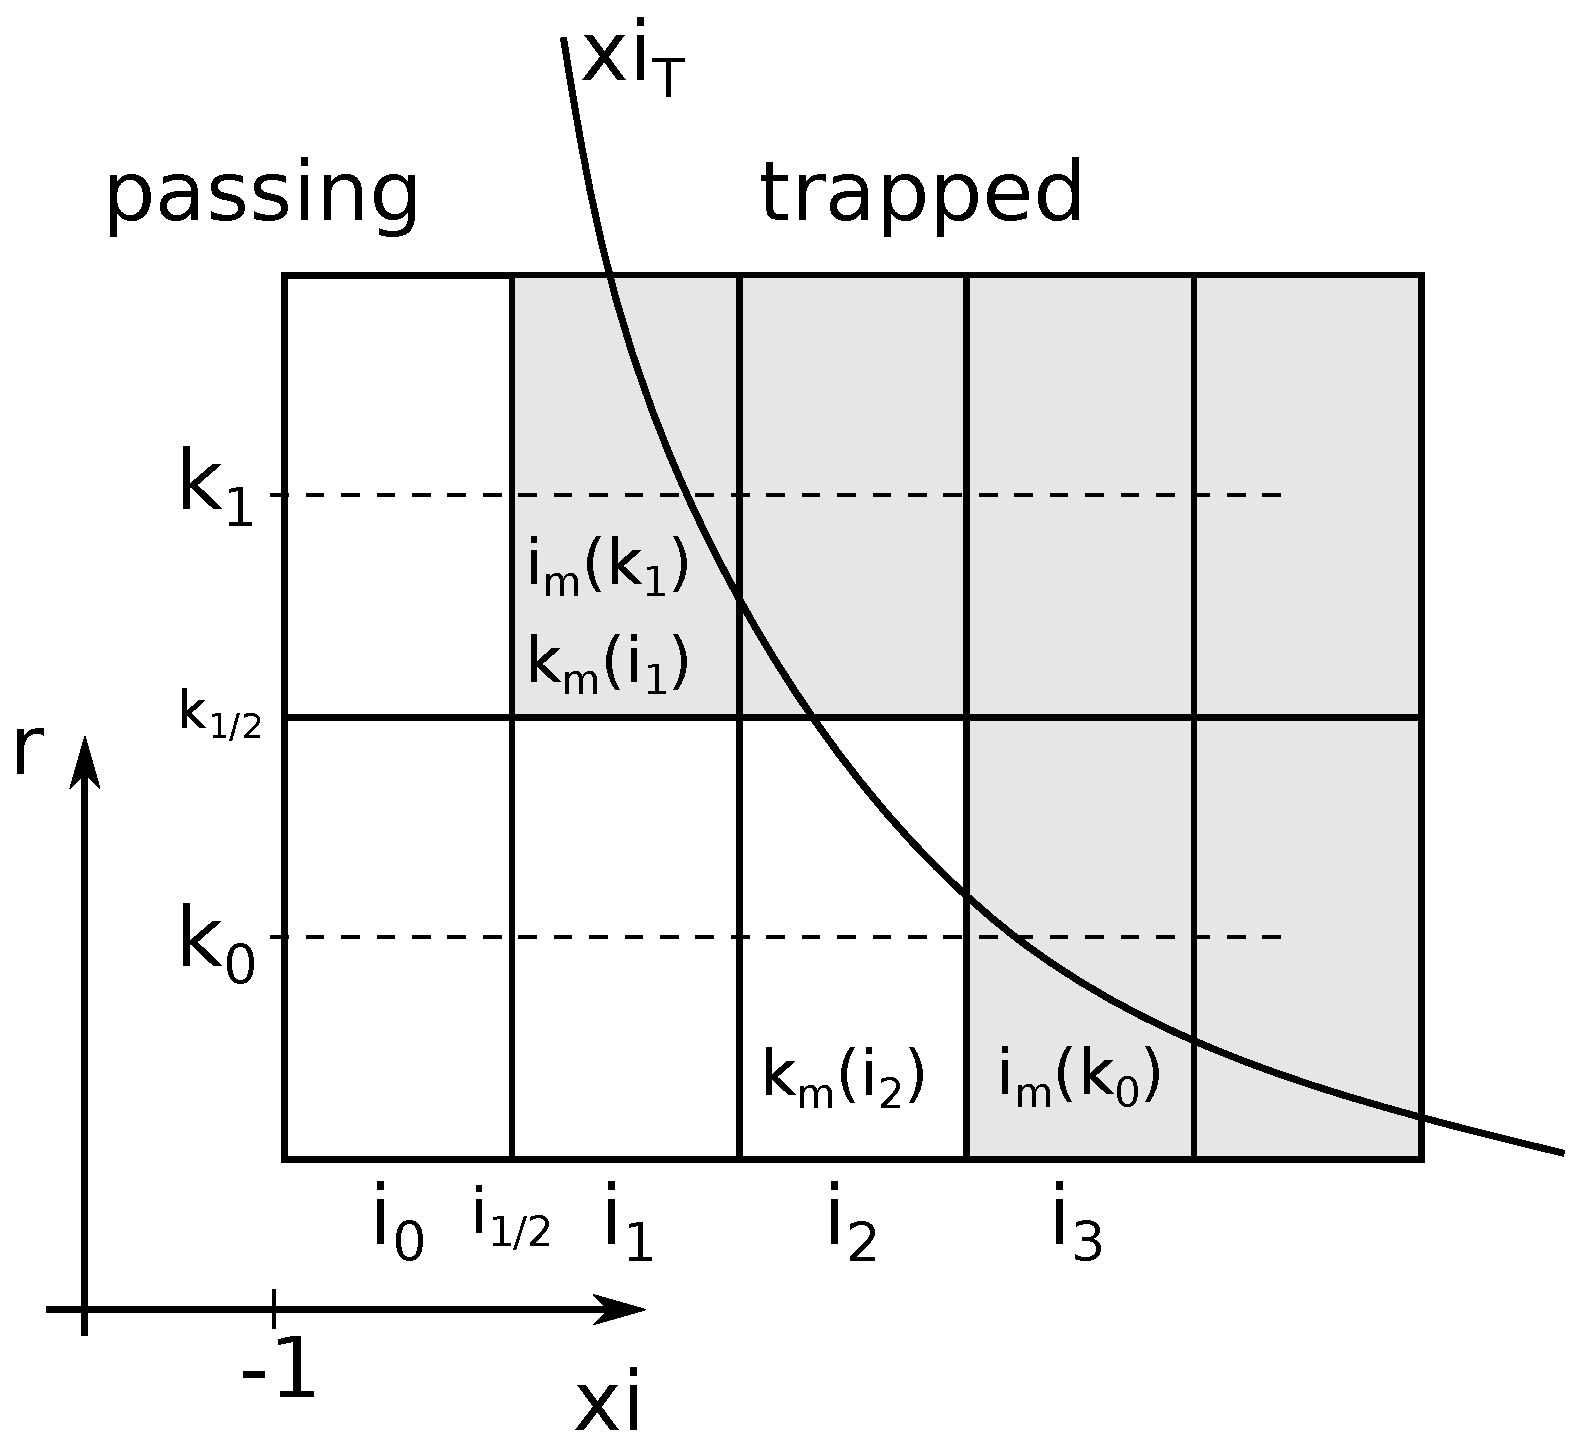
\includegraphics[width=0.9\textwidth,trim=-10mm 0 10mm 0]{trappedbc_fig}
\caption{Illustration of trapped-passing boundary and definition of special cells. Pitch fluxes into cells $i_m$ and radial fluxes into cells $k_m$ are moved to the mirrored cells. Shaded: cells where the distribution is not evolved by a kinetic equation but mirrored according to $f(\xi) = f(-\xi)$.}
\end{center}
\end{figure}

\newpage 

We define the bounce-integral of an arbitrary pitch-dependent quantity $X(\xi)$ 
\begin{align}
\{ X \}(\xi_0) = \int_0^{2\pi} \rd \varphi \int_0^{2\pi}\rd \zeta \times \begin{cases}
\int_{-\pi}^\pi \rd \theta \, \sqrt{g}X(\xi) & \text{passing}, \\
\int_{\theta_{b1}}^{\theta_{b2}} \rd \theta \, \sqrt{g}[X(\xi) + X(-\xi)]  & \text{trapped}, ~ \xi_0>0, \\
0 & \text{trapped}, ~ \xi_0\leq 0.
\end{cases}
\end{align}
where $\sqrt{g}$ is the jacobian of the coordinate system and $\theta_{b1},\,\theta_{b2}$ the two bounce points. Essentially, we don't describe trapped particles with negative $\xi_0$ as they are in fact the same as the corresponding particle with positive pitch (of the same magnitude) -- they are weighted with the entire trajectory bouncing back and forth. The distribution function is subject to the condition $f(-\xi_0) = f(\xi_0)$ inside the trapped region.
Furthermore, we define the bounce-integrated jacobian as
\begin{align}
\mathcal{V}' = \{1\}.
\end{align}

The kinetic equation (and distribution function) is discretized by integrating it over the cell centered at $(r_k,\,p_j,\,\xi_i)$ and approximating with a midpoint rule
\begin{align}
\int \rd \b{p} \rd \b{x}  f \approx f(r_k,\,p_j,\,\xi_i) \mathcal{V}'(r_k,\,p_j,\,\xi_i) \Delta r_k \Delta p_j \Delta \xi_i,
\end{align}
where we simply evaluate the integrand in the cell center.
This method is typically relatively accurate since $f$ is continuous and $\mathcal{V}'$ a smoothly varying function. However, in an inhomogeneous magnetic field there are three singular points in $\xi$ where this approximation is no longer good: on the trapped-passing boundary $\xi=\pm \xi_T$ where $\mathcal{V}'$ has a logarithmic singularity, and at $\xi=0$ where $\mathcal{V}'$ vanishes identically.

In these points, we may note that $f$ still varies relatively slowly, but \Vp{} does not. Then, we improve the accuracy (at some computational expense) by instead taking
\begin{align}
\int \rd \b{p} \rd \b{x}  f &\approx f(r_k,\, p_j ,\,\xi_i) \Delta r_k \Delta p_j \int_{\xi_i-\Delta \xi_i/2}^{\xi_i+\Delta \xi_i/2} \Vp(r_k,\,p_j,\,\xi) \,\rd\xi \nonumber \\
&\equiv f(r_k,\,p_j,\,\xi_i) \mathcal{V}'(r_k,\,p_j,\,\xi_i) \Delta r_k \Delta p_j \Delta \xi_i,
\end{align}
where we have simply redefined
\begin{align}
\Vp_i \mapsto \frac{1}{\Delta \xi_i}\int_{\xi_i-\Delta \xi_i/2}^{\xi_i+\Delta \xi_i/2} \Vp(r_k,\,p_j,\,\xi) \,\rd\xi 
\end{align}
at these three singular points, and where we can evaluate the (convergent) integral to any desired accuracy. Since \Vp{} is a nearly linear function of $\xi$ in a vicinity around $\xi=0$, for the cell surrounding this point we may take
\begin{align}
\Vp(r_k,\,p_j,\,\xi_i) \approx \frac{\xi_{i+1/2}^2}{2} \Vp(r_k,\,p_j,\,\xi_{i+1/2}), \quad \text{for } \xi_{i-1/2} < 0 < \xi_{i+1/2}.
\end{align}
The question may arise whether we shouldn't also integrate over $r$, as \Vp would vary sensitively also with respect to that. However, I suspect that since the $\xi$ integral resolves the singularity, the resulting averaged function is not as sensitive to radial variations and we can safely evaluate at cell center (in radius).

The same method as described here to evaluate \Vp should also be applied when evaluating bounce averages of various quantities in the singular points.

Let us have a closer look at the calculation of the cell average $\mathcal{V}'$. Consider an integration over an interval in $\xi_0$ ranging from $\xi_1$ to $\xi_2$, which contains the trapped-passing boundary $\xi_1 < \xi_T < \xi_2$. It is convenient to split this interval and consider separately the integrals on intervals $[\xi_1,\,\xi_T]$ in the trapped region, and $[\xi_T,\,\xi_2]$ in the passing region. 

Consider first the passing contribution, where we can simply change integration order
\begin{align}
\int_{\xi_T}^{\xi_2} \rd \xi_0 \, \mathcal{V}' = (2\pi)^2 \int_{-\pi}^\pi \rd \theta \, \int_{\xi_T}^{\xi_2} \rd \xi_0 \, \sqrt{g}.
\end{align}
The metric is given by
\begin{align}
\sqrt{g} &= \mathcal{J}\frac{B}{B\sub{min}}\frac{\xi_0}{\xi} = \mathcal{J}\left|\frac{\partial \xi}{\partial \xi_0}\right|, \\
\xi &= \text{sgn}(\xi_0)\sqrt{1-(1-\xi_0^2)\frac{B}{B\sub{min}}},
\end{align}
and the trapped-passing boundary is given by $\xi_T = \sqrt{1-B\sub{min}/B\sub{max}}$. Then,
\begin{align}
\int_{\xi_T}^{\xi_2} \rd \xi_0 \, \mathcal{V}' &= (2\pi)^2 \int_{-\pi}^{\pi} \rd \theta \, \mathcal{J} \left( \sqrt{ 1 - (1-\xi_2^2)\frac{B}{B\sub{min}}} - \sqrt{1-\frac{B}{B\sub{max}}}  \right) \nonumber \\
&= V' \langle F_2\rangle,
\end{align}
where $V'$ is VpVol, $\langle \rangle$ denotes the flux surface average and the function $F$ is given by
\begin{align}
F &= 2\pi \left( \sqrt{ 1 - (1-\xi_2^2)\frac{B}{B\sub{min}}} - \sqrt{1-\frac{B}{B\sub{max}}} \right) \nonumber \\
&= 2\pi \frac{B}{B\sub{max}} \frac{ 1 - (1-\xi_2^2)\frac{B\sub{max}}{B\sub{min}} }{ \sqrt{ 1 - (1-\xi_2^2)\frac{B}{B\sub{min}}} + \sqrt{1-\frac{B}{B\sub{max}}} }.
\end{align}
This form is convenient, since it can be expressed as a simple flux surface average. For the trapped contribution, the change of integration orders is less trivial, and we obtain
\begin{align}
\int_{\xi_1}^{\xi_T}\rd\xi_0 \,\mathcal{V}' &= 2(2\pi)^2 \int_{-\pi}^\pi \rd \theta \int_{\xi^\star}^{\xi_T} \rd \xi \, \sqrt{g}, \nonumber \\
\xi^\star &= \text{max}\left(\xi_1, \, \sqrt{1-\frac{B\sub{min}}{B(\theta)}}\right).
\end{align}
If we define the poloidal angles $\theta_{1l}$ and $\theta_{1u}$ such that $\sqrt{1-B\sub{min}/B(\theta_1)} = \xi_1$ and $\theta_{1l} < \theta\sub{min} < \theta_{1u}$ where $B\sub{min} = B(\theta\sub{min})$, the integral takes the form
\begin{align}
\int_{\xi_1}^{\xi_T}\rd\xi_0 \,\mathcal{V}' &=  2(2\pi)^2 \int_{-\pi}^\pi \rd \theta \,\mathcal{J}\sqrt{1-\frac{B}{B\sub{max}}} - 2(2\pi)^2 \int_{\theta_{1l}}^{\theta_{1u}}\rd \theta \, \sqrt{ 1 - (1-\xi_1^2)\frac{B}{B\sub{min}}}
\end{align}

\subsection*{Numerical description of flows}
Consider now an equation term describing a continuous flux in pitch
\begin{align}
\frac{1}{\mathcal{V}'}\frac{\partial \mathcal{V}' \Phi}{\partial \xi_0} ,
\end{align}
where $\Phi$ is some particle flux, typically originating from advection and diffusion of the distribution. We discretize the pitch coordinate with a finite volume treatment with cells centered on $\xi_i$, $i=1,\,2,\,...,\,N$ and associated cell faces $\xi_{i-1/2}$ and $\xi_{i+1/2}$ such that $\xi_i = (\xi_{i-1/2} + \xi_{i+1/2})/2$. The discretized form of the flux term in grid cell $i$ is given by
\begin{align}
\left(\frac{1}{\mathcal{V}'}\frac{\partial \mathcal{V}' \Phi}{\partial \xi_0} \right)_i 
	&= \frac{\mathcal{V}'_{i+1/2}\Phi_{i+1/2} - \mathcal{V}'_{i-1/2}\Phi_{i-1/2}}{\mathcal{V}'_i \Delta \xi_i} \\
\Delta \xi_i &= \xi_{i+1/2}-\xi_{i-1/2}
\end{align}
Because of the mirror symmetry between co-passing and counter-passing particles, we will assume that the particle flux which enters into the cell which contains the negative trapped-passing boundary $-\xi_T$ will be added into the cell containing $\xi_T$. We let $i_m$ denote the index of the cell containing $-\xi_T$, $i_p$ the cell containing $\xi_T$ and $i_0$ that containing $\xi_0$:
\begin{align}
\xi_{i_m-1/2} \leq -&\xi_T < \xi_{i_m+1/2}, \nonumber \\
\xi_{i_p-1/2} < {} & \xi_T \leq \xi_{i_p+1/2}, \nonumber \\
\xi_{i_0-1/2} \leq{} &0 < \xi_{i_0+1/2}.
\end{align}
Note that two or even all three of these indices can be the same. Our trapping condition is that
\begin{align*}
&\hspace{-7mm} \textbf{\emph{Fluxes into cells $i_m \leq i < i_0$ should be added into the cell $\hat{i}$ containing $-\xi_i$}} \\
& \hspace{-15mm}\textbf{\emph{ Equivalently, $- \xi_T < \xi_{i+1/2} < 0$: the upper cell face IsTrapped with negative pitch. }} \\
& \hspace{15mm} \textbf{\emph{ The distribution in these cells satisfies $f_i = f_{\hat i}$ }}
\end{align*}
Note that the condition $i_m \leq i < i_0$ is equivalent to $- \xi_T < \xi_{i+1/2} < 0$, i.e.~the upper cell face corresponds to a trapped orbit with negative pitch.
If $i_m=i_0$, nothing needs to be done except for the more careful determination of \Vp\! as described in the first section. Otherwise, the discretization of the flux in the $i_p$ cell is given by
\begin{align}
\left(\frac{1}{\mathcal{V}'}\frac{\partial \mathcal{V}' \Phi}{\partial \xi_0} \right)_{i_p} &=  \frac{\mathcal{V}'_{i_p+1/2}\Phi_{i_p+1/2} - \mathcal{V}'_{i_p-1/2}\Phi_{i_p-1/2} - \mathcal{V}'_{i_m-1/2}\Phi_{i_m-1/2}}{\mathcal{V}'_{i_p} \Delta \xi_{i_p}}, %\\
%\left(\frac{1}{\mathcal{V}'}\frac{\partial \mathcal{V}' \Phi}{\partial \xi_0} \right)_{i_0} &=  \frac{\mathcal{V}'_{i_0+1/2}\Phi_{i_0+1/2} - \mathcal{V}'_{i_0-1/2}\Phi_{i_0-1/2}}{\mathcal{V}'_{i_0}\Delta \xi_{i_0}} \nonumber \\
%&=\frac{\mathcal{V}'_{i_0+1/2}\Phi_{i_0+1/2} }{\mathcal{V}'_{i_0}\Delta \xi_{i_0}} ,
\end{align}
where we have added the particle flux $\Phi_{i_m-1/2}$ which goes from cell $i_m-1$ into cell $i_m$. This form ensures that no particle flux is lost across the internal boundaries.
%, and in the second term $\Vp_{i_0-1/2}$ vanishes because this point lies inside $-\xi_T < \xi < 0$ \textcolor{red}{(special case: unless the negative trapping region is covered inside the $i_0$ cell, ie $\xi_{i_0-1/2} \leq -\xi_T < 0 < \xi_{i_0+1/2}$, in which case there is no special $i_0$ case, as it is described by $i_m$.)}.
We don't solve an equation for the distribution in cell $i_m$, and instead impose mirror symmetry $f(\xi_{i_m}) = f(-\xi_{i_m})$; if there is no grid cell at $-\xi_{i_m}$ we interpolate linearly between the two closest points.

\subsubsection*{Radial flux}
Although we let the above considerations about the pitch-fluxes determine which cells are considered ``trapped'', the radial fluxes will need to be treated in a different way. The issue arises because, depending on magnetic field and radial resolution, the situation may occur where $(r_{k+1/2},\,\xi_{i_m-1})$ is a trapped orbit even though the cell is regarded as a ``passing'' (when we considered the pitch fluxes). In that case, $\mathcal{V}'=0$ in our approximation, yielding no flux out of the cell.

Therefore, analogous to the pitch case, we define $k_m$ as the index (at a given $\xi$ index $i$) for which ($r_{k_m+1/2},\,\xi_i$) is trapped. Radial fluxes into the $(k_m,\,i)$ cell should then be added into the cell $(k_m,\,i')$ where $i'$ is the cell containing $-\xi_i$.

\subsection*{Grid refinement}
For accuracy, it is probably good if the $i_m$ cells have as small a volume as possible. This is because the distribution in these cells are not followed dynamically (only mirrored), yet still are partially in the passing region where we wish to evolve the distribution. Therefore, the grid can be \emph{refined} by adding additional pitch grid points that tightly straddle the trapped-passing boundary, such that the cell volume $\mathcal{V}'_{kji_m} \Delta r_k \Delta p_j \Delta \xi_{i_m}$ becomes much smaller than adjacent cells.  Since we wish to avoid having cell faces too close to the trapped-passing region because the fluxes diverge there, it is good to center these additional cells on the trapped passing boundary and having the width sufficiently large that the `entire' singularity is captured (typically there is a distinct peak that has a full-width of $\Delta \xi \sim 0.05$. See figure 2 of how $\mathcal{V}'$ depends on $\xi$ in a magnetic geometry with circular flux surfaces. 


\begin{figure}[H]
\begin{center}
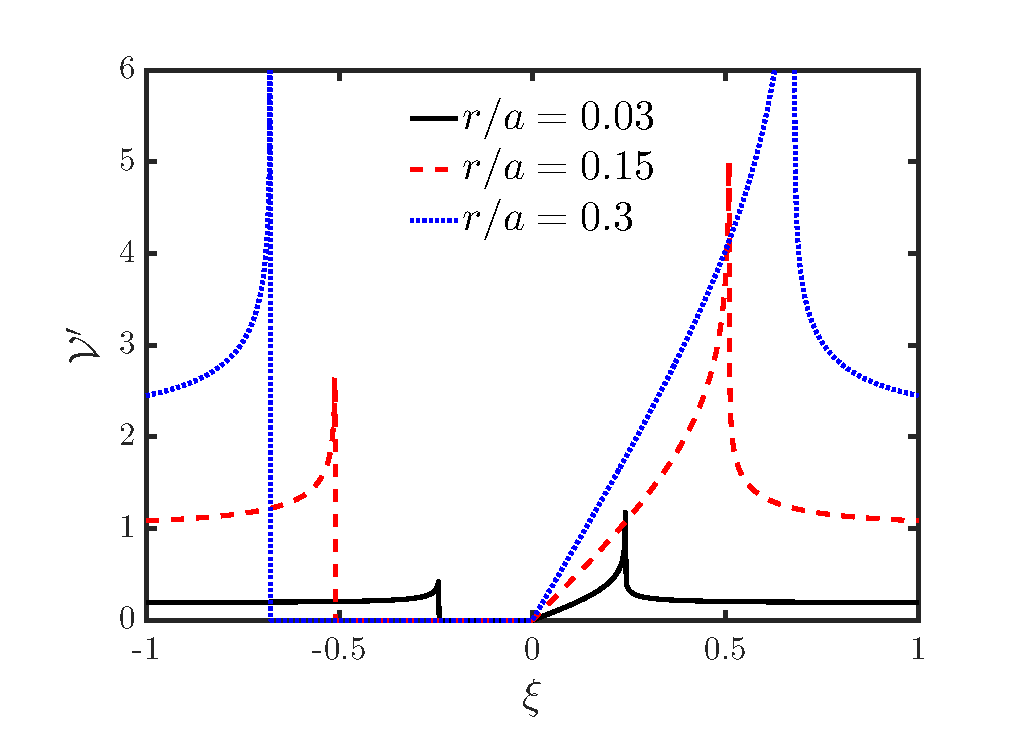
\includegraphics[width=1.02\textwidth,trim=0 0 0 20mm]{trappedbc_VpPlot}
\caption{Dependence of bounce averaged metric in a magnetic field with circular flux surfaces. The metric is normalized to the minor and major radius $R_0a$.}
\end{center}
\end{figure}

\begin{figure}[H]
\begin{center}
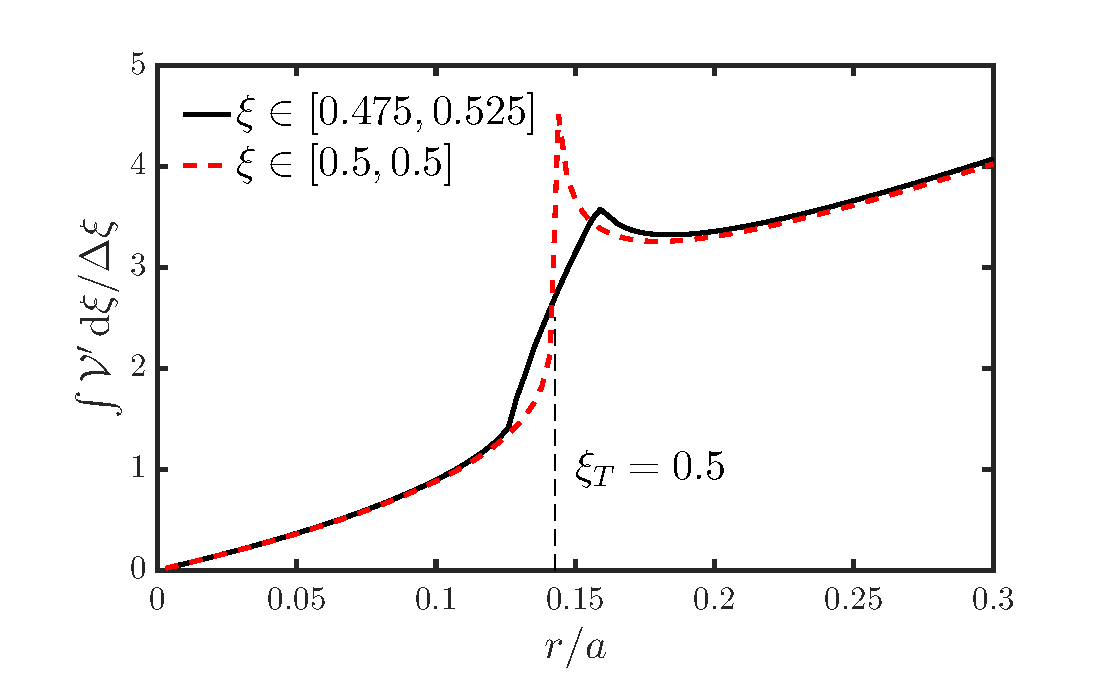
\includegraphics[width=1.02\textwidth,trim=0 0mm 0 10mm]{trappedbc_IntegratedVpPlot}
\caption{Radial dependence of $\mathcal{V}'$ when integrated over a narrow boundary layer cell with $\Delta \xi=0.05$ (compared with $\Delta\xi=0$ in red). Indicated with a dashed line is the radius where the trapped-passing boundary occurs in the cell center, at $\xi=0.5$. The metric is normalized to the minor and major radius $R_0a$.}
\end{center}
\end{figure}


Figure 3 shows the radial dependence of $\mathcal{V}'$ when integrated over such a narrow cell; because the result is relatively smoothly varying after the pitch integration has resolved the singularity, this justifies evaluating the pitch-averaged $\mathcal{V}'$ in $r_k$ rather than also integrating carefully over radius.

One way to construct a refined grid is therefore to:
\begin{enumerate}
\item Construct a regular grid with desired $\Delta \xi$ spacings according to the resolution needs of the problem.
\item For each radial grid point $k$, create two new pitch cells by adding two additional flux grid points at $\xi_{i_p\pm1/2} = \xi_T(r_k) \pm 0.025$ (but never below 0). {\bf \emph{If there already exists a grid point in this interval, remove it.}}
\item Add a flux grid point at $\xi=0$.
\item {\bf \emph{Redistribute all grid points in between the new boundary layer cells uniformly. (Optional) If the resulting grid spacing becomes smaller than half the original spacing, remove grid points.}}
\item Mirror the trapping region (including the boundary layer cell which extends beyond the boundary): for all $0 < \xi_i \leq \xi_T(r_k)+0.025$, create flux grid points at $-\xi_i$ (removing all previous points in this interval).
\end{enumerate}
The choice of $\Delta \xi = 0.05$ is arbitrary and could be tweaked. We could try setting it to a fraction of the local grid spacing (ie say $\Delta \xi/5$ or similar).
Figure 4 illustrates a refined version of the grid in figure 1.

\begin{figure}
\begin{center}
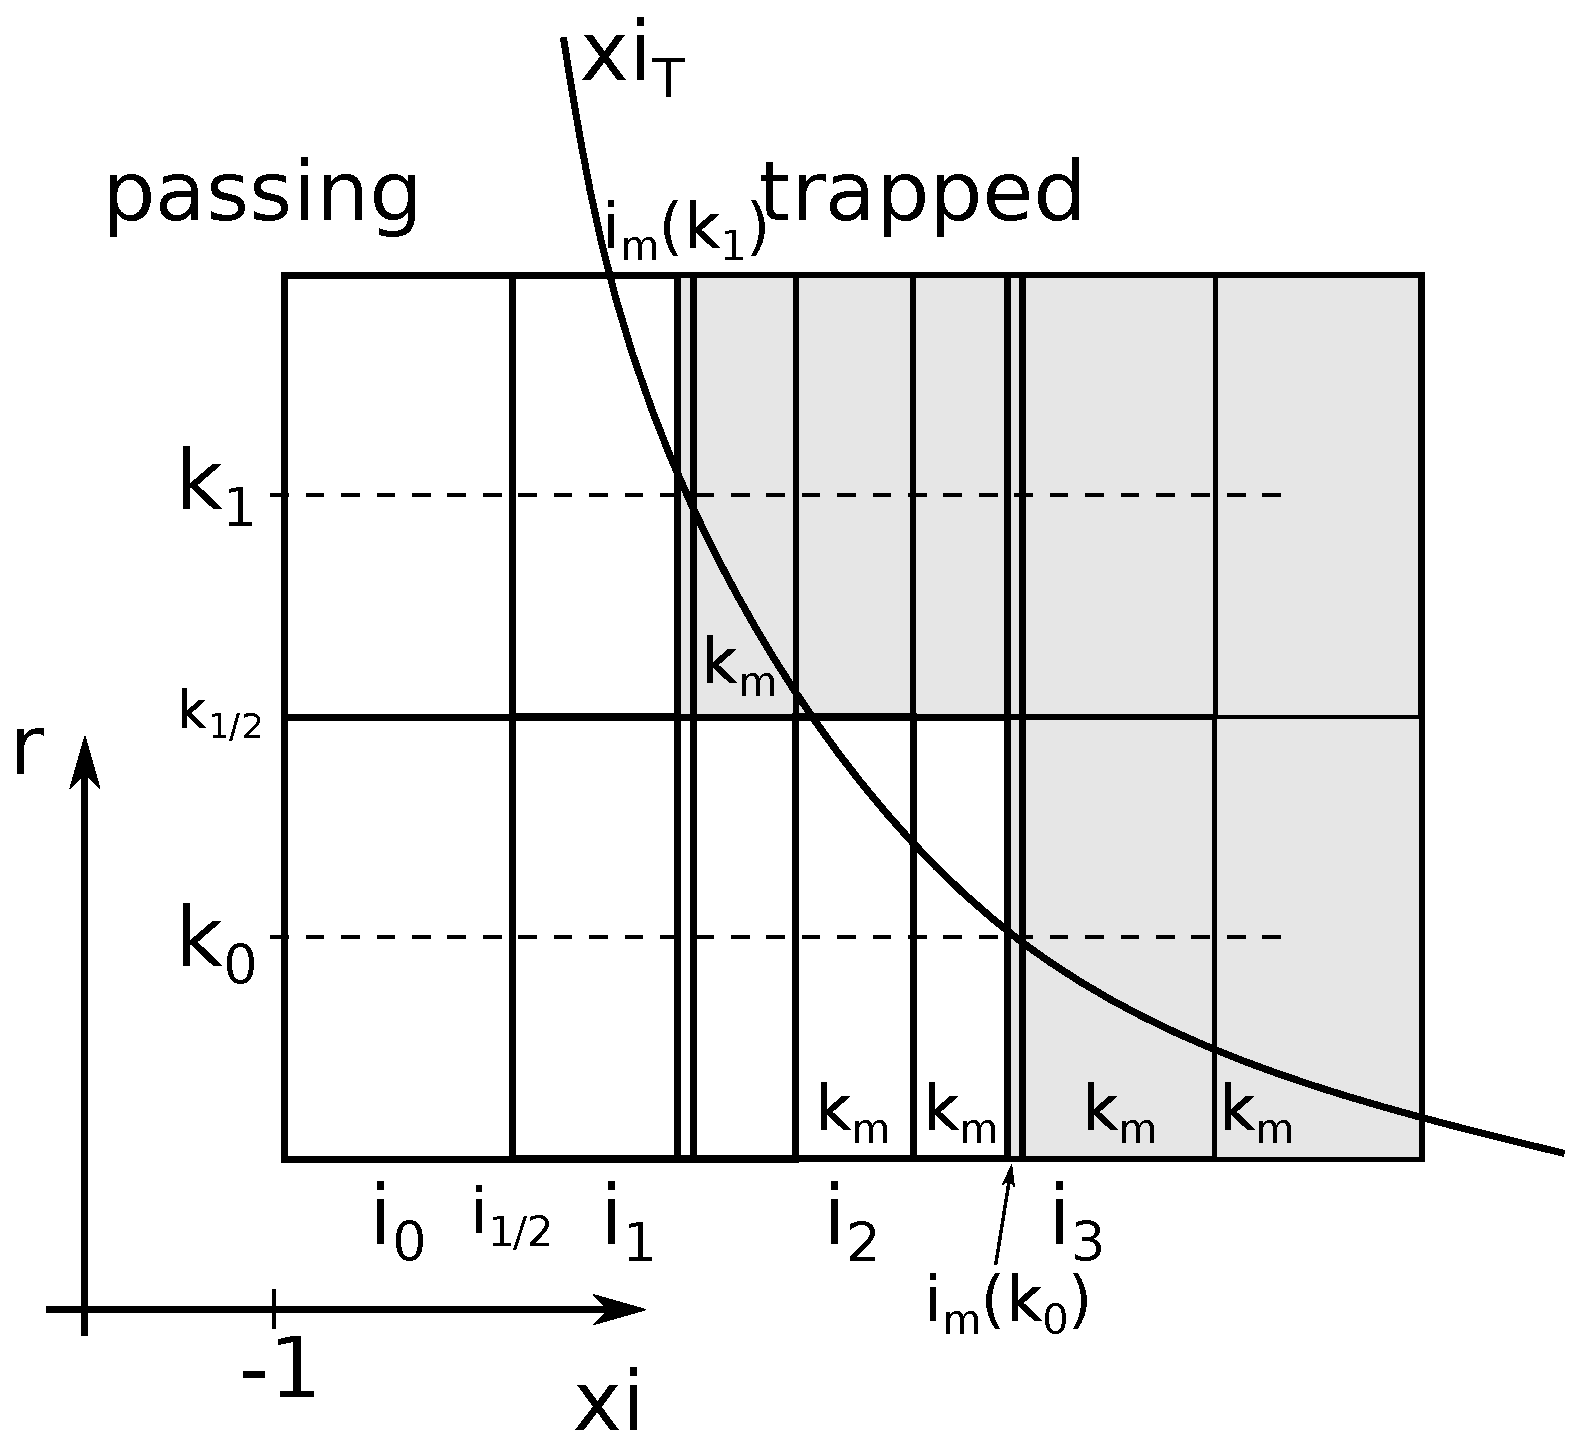
\includegraphics[width=1.0\textwidth,trim=10mm 0 10mm 0]{trappedbc_fig_refined}
\caption{Illustration of the finite-volume mesh from figure 1, after performing a refinement of the pitch grid such that the cells containing the trapped-passing boundary in radial cell centers are made to have small volume by the addition of boundary-layer cells. }
\end{center}
\end{figure}

\subsubsection*{Optional: refined radial grid}
In order to better capture trapping-detrapping by radial transport, we could also refine the radial grid in order to reduce the volume of all $k_m$ cells. In that case, add:
\begin{enumerate}
\item[6.] For each cell center $\xi_i \neq \{0,\,\xi_T\}$, there exists a radius $r^\star_i$ such that $\xi_T(r^\star_i) = \xi_i$. Add radial flux grid points at $r_{k_m \pm 1/2} = r^\star_i \pm d$ (unless $r_{k_m+1/2}>r\sub{max}$), where $d$ is some small radius (say, a fraction of $\Delta r$). {\bf \emph{If there already exists a grid point in this interval, remove it.}}
\end{enumerate} 
We do not need to add new radial grid points for those $\xi$ in boundary layer cells at $\xi_T$ since these cells already have small volume.

This procedure will require a grid resolution $n_r \sim n_\xi$ which may or may not be feasible. It may be argued that the pitch-angle dynamics is the most important to capture, since pitch-angle scattering is always a dominant effect whereas the radial transport is typically applied ad-hoc and is not based on first principles. Therefore pitch refinement should probably be prioritized over radial grid refinement.



\end{document}


\subsubsection*{Radial fluxes, and $V_p$ reconsidered}
The radial flux turns out to be really challenging and highlights a flaw with our current method. Consider the behaviour of a radial flux term
\begin{align}
\frac{\partial f}{\partial t} = \frac{1}{\mathcal{V}'}\frac{\partial \mathcal{V}'\Phi}{\partial r}
\end{align} 
where we let the pitch be negative.
In our FVM discretization, this becomes
\begin{align}
\frac{\partial f_{kji}}{\partial t} = \frac{\mathcal{V}'(r_{k+1/2},p_j,\,\xi_i)\Phi(r_{k+1/2},\,p_j,\,\xi_i) - [\text{$(k-1/2)$-term}]}{\mathcal{V}'(r_k,p_j,\xi_i)}.
\end{align}
Now, even though the $kji$ cell that we consider may contain only passing orbits, we may have the situation where $(k+1)ji$ is (deeply) trapped such that $\mathcal{V}'(r_{k+1/2},p_j,\,\xi_i)=0$, and may even be zero at $\xi_{i-1}$. In this case there would be no radial flux in the discretized equation, even though there would be in the continuous limit.

Let us have a more careful look a the discretization. Integrating the equation over the volume of a cell yields
\begin{align}
\frac{\partial}{\partial t}\int_{kji}\rd r \rd p \rd \xi \,\mathcal{V}'f = \int \rd p \int \rd \xi \, \mathcal{V}'(r_{k+1/2})\Phi(r_{k+1/2}) - ...|_{k-1/2}.
\end{align}
Now, since the distribution is continuous, we will use our usual approximation of evaluating it on the cell and face centers, but we will be more careful with the metric and advection-diffusion terms which have singularities, discontinuities and cusps in the ($r$-$\xi$) plane. Because nothing exciting happens in $p$, we will treat it like the distribution and evaluate it at the centers. Using an advection term as an example, $\Phi = Af$, we then get
\begin{align}
\frac{\partial f_{kji}}{\partial t} \int \rd r \rd \xi \, \mathcal{V}'(r,\,p_j,\,\xi) = f_{(k+1/2)ji} \int \rd \xi \, \mathcal{V}' A (r_{k+1/2}, p_j, \xi) - ...|_{k-1/2}.
\end{align}
Thus, the equation becomes
\begin{align}
\frac{\partial f_{kji}}{\partial t} \equiv \frac{\mathcal{V'}_{(k+1/2)ji}\{A\}_{(k+1/2)ji} f_{(k+1/2)ji} - ...|_{k-1/2}}{\mathcal{V'}_{kji} \Delta r_k}
\end{align}
as usual but where
\begin{align}
\mathcal{V'}_{kji} &= \frac{1}{\Delta r_k \Delta \xi_i} \int_{r_{k-1/2}}^{r_{k+1/2}} \rd r \int_{\xi_{j-1/2}}^{\xi_{j+1/2}} \rd \xi \, \mathcal{V}'(r,\,p_j,\,\xi) , \nonumber \\
\mathcal{V'}_{(k+1/2)ji} &= \frac{1}{\Delta \xi_i} \int_{\xi_{j-1/2}}^{\xi_{j+1/2}} \rd \xi \, \mathcal{V}'(r_{k+1/2},p_j,\xi).
\end{align}
Now, away from the trapped-passing boundary (or $\xi=0$) the integrals are slowly varying and our regular approximation of using the midpoint rule for the integrals works well. However, near these points we must be more careful. In order to avoid the above-mentioned issue of disappearing radial flux, we can approximate the radial integral with a trapezoid rule,
\begin{align}
\mathcal{V}'_{kji} &\approx  \frac{1}{\Delta r_k \Delta \xi_i} \int_{\xi_{j-1/2}}^{\xi_{j+1/2}} \rd \xi \, \Delta r_k\frac{\mathcal{V}'(r_{k+1/2},\,p_j,\,\xi)+\mathcal{V}'(r_{k+1/2},\,p_j,\,\xi) }{2}  \nonumber \\
&= \frac{\mathcal{V}'_{(k+1/2)ji} + \mathcal{V}'_{(k-1/2)ji}}{2},
\end{align}
whereas the the pitch integral should ideally be evaluated with an accurate quadrature that can handle the logarithmic singularity on the trapped-boundary and captures the value within a small error. With this change, it is guaranteed that if $\mathcal{V}'_{k+1/2}$ is non-zero (so that there is a radial flux), then so is $\mathcal{V}'_k$ and $\mathcal{V}'_{k+1}$.

For a pitch-angle flux, the discretized equation instead takes the form
\begin{align}
\frac{\partial f_{kji}}{\partial t} \equiv \frac{\mathcal{V'}_{kj(i+1/2)}\{A\}_{kj(i+1/2)} f_{kj(i+1/2)} - ...|_{i-1/2}}{\mathcal{V'}_{kji} \Delta \xi_i},
\end{align}
where
\begin{align}
\mathcal{V}'_{kj(i+1/2)} = \frac{1}{\Delta r_k} \int_{r_{k-1/2}}^{r_{k+1/2}} \rd r \, \mathcal{V}'(r,p_j,\xi_{i+1/2}).
\end{align}
This radial integral needs to be carried out with a high-accuracy quadrature since it also contains a singularity on the trapped-passing boundary.

With these changes, we end up with the same picture as previously, but we should probably define $i_m$ as the first cell for which the trapped-passing boundary intersects the left cell face (ie for which $\xi_{i_m+1/2} > - \xi_{T,k+1/2}$)
as the cell for which $\mathcal{V}'_{kj(i_m+1/2)} = 0$
\vspace{20mm}

Let us assume that for all $i_1 < i < i_2$, the distribution is taken to satisfy $f(\xi_i) = f(-\xi_i)$ because they describe counter-passing ($\xi<0$) particles which would be double counted, such that the total particle density is given in terms of
\begin{align}
n \propto \left(\sum_{i=1}^{i_1} + \sum_{i=i_2}^N\right) \mathcal{V}'_i \Delta \xi_i f_i.
\end{align}
\textcolor{red}{[The below is faulty, skip to next section]} Flux conservation then demands that
\begin{align}
\text{[external flux]} &= \left(\sum_{i=1}^{i_1} + \sum_{i=i_2}^N\right) \left(\frac{1}{\mathcal{V}'}\frac{\partial \mathcal{V}' \Phi}{\partial \xi_0} \right)_i \nonumber \\
&= \mathcal{V}'_{i_1+1/2} \Phi_{i_1+1/2} - \mathcal{V}'_{i_2-1/2} \Phi_{i_2-1/2}  + \text{[external flux]}.
\end{align}
Flux conservation therefore demands that
\begin{align}
\mathcal{V}'_{i_1+1/2} \Phi_{i_1+1/2}  =  \mathcal{V}'_{i_2-1/2} \Phi_{i_2-1/2}.
\end{align}
This will not hold in general for non-trivial orbits, and therefore the only way to satisfy this generally is if $i_1$ and $i_2$ are the first indices such that
\begin{align}
\xi_{i_1+1/2} &\geq -\xi_T, \nonumber \\
\xi_{i_2+1/2} &\geq 0.
\end{align}
However, an issue arises if $\xi_{i_1}$ or $\xi_{i_2}$ lie in the interval $-\xi_T \leq \xi \leq 0$, since we assumed that this was not the case, but this is not guaranteed to hold for general grids from the constraints obtained above.
This simplest FVM discretization outlined here therefore seems to put an additional constraint on the grids that we choose for our problem:
\begin{align}
&\text{The pitch grid must satisfy} \nonumber \\
&\hspace{10mm} \xi_{i_1} < -\xi_T \leq \xi_{i_1 + 1/2}, \nonumber \\
&\hspace{6mm} \xi_{i_2-1/2} \leq 0 < \xi_{i_2},  \\
&\text{for some indices $i_1$ and $i_2$ for $\xi_T$ at all radii.} \nonumber
\end{align}

\subsection*{New attempt at Numerical description of flows}
The previous attempt was flawed, because we obtained only a trivial solution where the fluxes vanished such that the solution for $\xi<-\xi_T$ completely decoupled from the solution at $\xi>0$. In reality, we want a non-zero flux to enter the $-\xi_T$ cell and enter directly into the mirrored $\xi_T$ cell. That is, we assume that there is some index $i_3$ which is a cell containing $\xi_T$, to which we add the flux $\mathcal{V}'_{i_1+1/2}\Phi_{i_1+1/2} \neq 0$.

In this case, we modify the above. We require that the pitch grid must satisfy
\begin{align}
&\xi_{i_1+1/2} < -\xi_T \leq \xi_{i_1 + 1}, \nonumber \\
&\xi_{i_2-1/2} \leq  0 < \xi_{i_2}
\end{align}
for some indices $i_1$ and $i_2$ for $\xi_T$ at all radii ($i_1$ and $i_2$ can and typically will be different at different radii) , and we set
\begin{align}
\left(\frac{1}{\mathcal{V}'}\frac{\partial \mathcal{V}' \Phi}{\partial \xi_0} \right)_{i_3} 
	=  \frac{\mathcal{V}'_{i_3+1/2}\Phi_{i_3+1/2} - \mathcal{V}'_{i_3-1/2}\Phi_{i_3-1/2} - \mathcal{V}'_{i_1+1/2}\Phi_{i_1+1/2}}{\mathcal{V}'_{i_3} \Delta \xi_{i_3}}.
\end{align}
A seemingly attractive solution is to choose a pitch grid such that there are always grid points satisfying $\xi_T = \xi_{i_3} = -\xi_{i_1+1}$ and $\xi_{i_2-1/2}=0$, e.g. a cell interface at $\xi=0$ and cell centers on the trapped-passing boundary $\pm \xi_T$ at each radius. This will require the resolution to at least match the number of radial grid points in the simulation, but that is probably not too big of a restriction (since the trapping region will require quite some number of grid points to resolve regardless).









\newpage
Let us assume that a trapping region covers all $-\xi_T < \xi < \xi_T$. Let us denote $i^\star$ and $i_0$ as the last indices $i$ for which 
\begin{align}
\xi_{i^\star+1/2} &\leq -\xi_T, \\
\xi_{i_0-1/2} &\leq 0.
\end{align}
We define that for all $i^\star < i < i_0$, $\mathcal{V}'_i=0$ and 

Flux conservation demands that
\begin{align}
\text{[External flux]} &= \sum_i \mathcal{V}'_i \Delta \xi_i \left(\frac{1}{\mathcal{V}'}\frac{\partial \mathcal{V}' \Phi}{\partial \xi_0} \right)_i 
= \left(\sum_{i=1}^{i^\star}  + \right)
\end{align}
